\documentclass[12pt]{article}
\usepackage[utf8]{inputenc}
\usepackage{graphicx}
\usepackage[a4paper,width=150mm,top=25mm,bottom=25mm]{geometry}
\title{

\\
{COS 301 User Stories}
}

\author{Ctrl Alt Defeat}

\begin{document}

\begin{titlepage}
    \centering



    \vspace{2cm}
    \hrulefill\\
    \vspace{1cm}
    {\Huge\bfseries SRS Documentation v3.0}

    \vspace{1cm}

    {\Large Software Requirements Specification Document for\\Domain Pulse}\\
    \vspace{1cm}
    \hrulefill\\

    \vfill

    {\large Ctrl Alt Defeat}

    \vspace{1cm}

    {\large 2023/07/31}\\
    %    \vspace{1cm}
    %    \vspace{1cm}
    %    
\includegraphics[width=10cm]{../../Images/dpLogo.png}
    %    \vspace{1cm}\\
    %    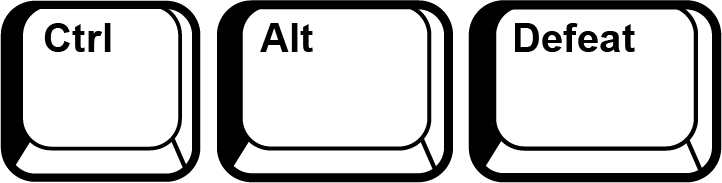
\includegraphics[width=6cm]{../../Images/cadLogo.png}

\end{titlepage}



\tableofcontents

\newpage


\section{User Stories}
\subsection{First Iteration}
\begin{table}[htbp]
\caption{User Story: Add a domain}
\begin{tabular}{|p{0.45\textwidth}|p{0.45\textwidth}|}
\hline
\textbf{User Story} & As a user/business manager, I want to add a domain (business, product, etc...) to my list of domains, so that I can view and track customers' sentiment of it. \\
\hline
\textbf{Acceptance Criteria} & 
Given that I provided the name of the domain I wish to track,\\
& When I click the 'add domain' button,\\
& Then the domain is added to my list. \\
\hline
\end{tabular}
\end{table}

\begin{table}[htbp]
\caption{User Story: Remove a domain}
\begin{tabular}{|p{0.45\textwidth}|p{0.45\textwidth}|}
\hline
\textbf{User Story} & As a user/business manager, I want to remove a domain (business, product, etc...) from my list of domains, so that I can remove unimportant or unneeded domains. \\
\hline
\textbf{Acceptance Criteria} & 
Given that I have selected the domain I wish to remove,\\
& When I click the 'remove domain' button,\\
& Then the domain is removed from my list. \\
\hline
\end{tabular}
\end{table}

\begin{table}[htbp]
\caption{User Story: Selecting a website theme}
\begin{tabular}{|p{0.45\textwidth}|p{0.45\textwidth}|}
\hline
\textbf{User Story} & As a user, I want to change the theme to light or dark mode for my personal preference, so that I can more enjoy my use of the web-app. \\
\hline
\textbf{Acceptance Criteria} & 
Given that I am within the web-app,\\
& When I click the 'Change Theme' button,\\
& Then the theme of the page is changed. \\
\hline
\end{tabular}
\end{table}
\begin{table}[htbp]
\caption{User Story: Log out of an account}
\begin{tabular}{|p{0.45\textwidth}|p{0.45\textwidth}|}
\hline
\textbf{User Story} & As a user, I want to log out of my account, so that I can log in on another or have more security of others not viewing my domains. \\
\hline
\textbf{Acceptance Criteria} & 
Given that I am currently signed into an account,\\
& When I click the 'Sign Out' button,\\
& Then I am signed out of my account and placed on the login page. \\
\hline
\end{tabular}
\end{table}
\begin{table}[htbp]
\caption{User Story: Add a source}
\begin{tabular}{|p{0.45\textwidth}|p{0.45\textwidth}|}
\hline
\textbf{User Story} & As a user/business manager, I want to add a source (Twitter, Instagram, etc...) for sentiment data to my list of sources, so that I can view and track customers' sentiment on said source. \\
\hline
\textbf{Acceptance Criteria} & 
Given that I provided the name/link to the source I wish to use,\\
& When I click the 'add source' button,\\
& Then the source is added to my list of sources. \\
\hline
\end{tabular}
\end{table}

\begin{table}[htbp]
\caption{User Story: Select a domain}
\begin{tabular}{|p{0.45\textwidth}|p{0.45\textwidth}|}
\hline
\textbf{User Story} & As a user/business manager, I want to select a domain (business, product, etc...) from my list of domains, so that I can view and track customers' sentiment regarding it and other pieces of meta-data regarding the sentiment. \\
\hline
\textbf{Acceptance Criteria} & 
Given that I have the domain I wish to view in my list of domains,\\
& When I click the domain's name in the list,\\
& Then the sources from where I pull data from are listed and the overall sentiment is displayed. \\
\hline
\end{tabular}
\end{table}

\begin{table}[htbp]
\caption{User Story: Register an account}
\begin{tabular}{|p{0.45\textwidth}|p{0.45\textwidth}|}
\hline
\textbf{User Story} & As a user, I want to create an account, so that I help my domains perform better by understanding if customers are satisfied by tracking customer sentiment. \\
\hline
\textbf{Acceptance Criteria} & 
Given that I have provided my email and password on the 'register' page,\\
& When I click the 'Register' button,\\
& Then my account is created and I am logged in. \\
\hline
\end{tabular}
\end{table}

\begin{table}[htbp]
\caption{User Story: Update Password}
\begin{tabular}{|p{0.45\textwidth}|p{0.45\textwidth}|}
\hline
\textbf{User Story} & As a user, I want to update my password, so that I can ensure the safety of my account or change it to one I shall remember. \\
\hline
\textbf{Acceptance Criteria} & 
Given that I am logged into an account,\\
& When I click the 'Update Password' button,\\
& Then I am prompted to verify by email if I want to update my password and enter my new password. \\
\hline
\end{tabular}
\end{table}
\begin{table}[htbp]
\caption{User Story: Remove a source}
\begin{tabular}{|p{0.45\textwidth}|p{0.45\textwidth}|}
\hline
\textbf{User Story} & As a user/business manager, I want to remove a source (Twitter, Instagram, etc…) for sentiment data from my list of sources, so as to remove an unhelpful or unwanted source of data. \\
\hline
\textbf{Acceptance Criteria} & 
Given that I have selected the source I wish to remove,\\
& When I click the 'remove source' button,\\
& Then the source is removed from my list of sources. \\
\hline
\end{tabular}
\end{table}

\begin{table}[htbp]
\caption{User Story: Select a domain}
\begin{tabular}{|p{0.45\textwidth}|p{0.45\textwidth}|}
\hline
\textbf{User Story} & As a user/business manager, I want to select a domain (business, product, etc...) from my list of domains, so that I can view and track customers' sentiment regarding it. \\
\hline
\textbf{Acceptance Criteria} & 
Given that I have the domain I wish to view in my list of domains,\\
& When I click the domain's name in the list,\\
& Then display the overall sentiment and list of sources selected for that domain. \\
\hline
\end{tabular}
\end{table}

\begin{table}[htbp]
\caption{User Story: Log into an account}
\begin{tabular}{|p{0.45\textwidth}|p{0.45\textwidth}|}
\hline
\textbf{User Story} & As a user, I want to log into my account, so that I help my domains perform better by understanding if customers are satisfied by tracking customer sentiment. \\
\hline
\textbf{Acceptance Criteria} & 
Given that I am not currently signed into an account, on the 'log-in' page and have my account details entered,\\
& When I click the 'Log In' button,\\
& Then I am logged into my account that stores my previously created domains and sources. \\
\hline
\end{tabular}
\end{table}

\begin{table}[htbp]
\caption{User Story: Forgot Password}
\begin{tabular}{|p{0.45\textwidth}|p{0.45\textwidth}|}
\hline
\textbf{User Story} & As a user, I want to update my password, so that I can change it to one I shall remember and access my account. \\
\hline
\textbf{Acceptance Criteria} & 
Given that I am on the log-in screen,\\
& When I click the 'Forgot Password' button,\\
& Then I am prompted to verify by email if I want to update my password and enter my new password. \\
\hline
\end{tabular}
\end{table}

\begin{table}[htbp]
\caption{User Story: Select a source}
\begin{tabular}{|p{0.45\textwidth}|p{0.45\textwidth}|}
\hline
\textbf{User Story} & As a user/business manager, I want to select a source (Twitter, Facebook, etc...) from my list of sources for a domain, so that I can view and track customers' sentiment regarding my domain within the source. \\
\hline
\textbf{Acceptance Criteria} & 
Given that I have selected a domain and have provided sources for said domain,\\
& When I click the source in the list,\\
& Then the overall sentiment specific to the source is displayed. \\
\hline
\end{tabular}
\end{table}

\begin{table}[htbp]
\caption{User Story: Select a statistic}
\begin{tabular}{|p{0.45\textwidth}|p{0.45\textwidth}|}
\hline
\textbf{User Story} & As a user/business manager, I want to select a statistic (sentiment or metadata) from all available statistics, so that I can gain a better insight into how that statistic compares to other statistics and how it affects the overall sentiment. \\
\hline
\textbf{Acceptance Criteria} & 
Given that sentiment analysis has been performed,\\
& When I click on a specific statistic,\\
& Then a visualization of the statistic is displayed. \\
\hline
\end{tabular}
\end{table}

\begin{table}[htbp]
\caption{User Story: View source data}
\begin{tabular}{|p{0.45\textwidth}|p{0.45\textwidth}|}
\hline
\textbf{User Story} & As a user/business manager, I want to be able to see examples of data that was retrieved from my sources, so that I can confirm that the correct source was specified and correctly retrieved. \\
\hline
\textbf{Acceptance Criteria} & 
Given that sentiment analysis has been performed,\\
& When I am viewing the source of a domain,\\
& Then the raw source data is also displayed. \\
\hline
\end{tabular}
\end{table}

\begin{table}[htbp]
\caption{User Story: View source data sentiments}
\begin{tabular}{|p{0.45\textwidth}|p{0.45\textwidth}|}
\hline
\textbf{User Story} & As a user/business manager, I want to be able to see what the application predicts people think based on what they have said, so that I can confirm the validity of the application’s predictions and trust the system. \\
\hline
\textbf{Acceptance Criteria} & 
Given that sentiment analysis has been performed,\\
& When I am viewing the examples raw source data of a domain,\\
& Then the predicted sentiment is displayed along with it. \\
\hline
\end{tabular}
\end{table}
\newpage
\subsection{Later Iterations}
\begin{table}[htbp]
\caption{User Story: View Time Series data}
\begin{tabular}{|p{0.45\textwidth}|p{0.45\textwidth}|}
\hline
\textbf{User Story} & As a user/business manager, I want to view the time series data of a domain's sentiment from customers, so that I can understand when customers most enjoyed or disliked my product. \\
\hline
\textbf{Acceptance Criteria} & 
Given that I have selected the domain I wish to see time series data on,\\
& When I click the 'Time Series' button,\\
& Then the page displays a graph of customer sentiment of the selected domain over a period of time. \\
\hline
\end{tabular}
\end{table}


\end{document}
